\documentclass{main.tex}[subfiles]
\begin{document}
\section{Метод полуконтролируемого обучения с автоматическим исправлением ошибок}
% TODO describe why design is like this (? tell about IOvo's research, about my thoughts on recto/verso comparison, classic OCR)

Поскольку мы не ограничены в выборе текстов для создания набора данных, пусть это будут художественные произведения, электронные варианты которых можно использовать для сравнения с результатом автоматической разметки.
Тогда процесс исправления неточностей будет заключаться в поиске сходства между распознанным текстом и оригиналом, и исправления в тех местах, где сходство нарушается.

\subsection{Предварительная обработка текста}\label{subsection:preprocessing}

Исходные данные для алгоритма исправления ошибок -- текст, полученный в результате распознавания (буквы, другие знаки, соответствующие символам азбуки Брайля, и пробелы), а также первоначальный электронный текст (буквы в верхнем и нижнем регистре, цифры и специальные символы).
% TODO describe grade 1
Чтобы каждая позиция в выравнивании соответствовала одному брайлевскому символу, референсная строка преобразуется: вместо символа троеточия вставляются три точки, унифицируется вид кавычек; буквы расширенной латиницы, отсутствующие в английском языке, заменяются латиницей (например, <<\'o>> $\rightarrow$ <<o>>) и так далее.

\subsection{Построение выравнивания}
Будем называть \emph{референсом (reference)} исходный текст и \emph{запросом (query)} строку, полученную в результате распознавания страницы (эти термины используются в биоинформатике, в задаче нахождения сходства между биологическими последовательностями).
Пусть эти две строки содержат только символы из некоторого алфавита $\mathcal A $. Введём символ \emph{пробела}: $ \ast \notin \mathcal A $.

\emph{Выравниванием} будем называть две строки одинаковой длины, полученные из референса и запроса вставкой нужного количества символов $\ast$ на некоторых позициях.
Выравнивание задаёт соответствие между символами двух строк с одинаковыми индексами (говорят, что символ из одной строки \emph{выравнивается} на другой); цель -- поиск наилучшего соответствия, содержащего как можно меньше пропусков и как можно больше попарных совпадений символов.

Ситуацию, когда два соответствующих символа в выравнивании различные и оба не являются пропусками, называют \emph{несовпадением (mismatch)}.
Если символ референса выравнивается на пропуск, это называют \emph{выпадением (deletion)}; выравнивание символа запроса на пробел -- \emph{вставка (insertion)}.
В нашей задаче, построив выравнивание, можно скорректировать метку класса в случае несовпадения или удалить метку в случае вставки.
Найденные выпадения никак не исправляются, поскольку мы не знаем, в каком месте изображения находится выпавший символ; в некоторых случаях можно попытаться определить место, где находится выпавшая буква, исходя из пространственного расположения соседних символов, но это выходит за рамки данной работы. \\

Похожие методы исправления символов ранее были разработаны для обычных программ распознавания текста по изображениям \cite{muller2021word_aln}.

\subsubsection{Поиск регионов интереса. Хэширование}

% TODO formulas: q-gram filtering, ...?

Поскольку каждая страница занимает малую часть исходного текста, и при этом неизвестно, какую именно, первый этап выравнивания -- поиск регионов интереса.
Под \emph{регионом интереса} будем понимать такой подотрезок референса, который, по нашему предположению, целиком содержит исходный текст, из которого в результате внесения ошибок получается запрос.

Будем искать регионы с помощью создания индекса $k$-кортежей референса.
\emph{k-кортеж} -- это любая строка длины $k$ над алфавитом $ \mathcal A  \cup \{ \ast \} $.

\begin{enumerate}[noitemsep]
    \item Максимальное число знаков в брайлевской строке -- 40, строк на странице -- 25, т. е. не более 1000 знаков на странице.
    Разделим референс на участки длиной 250 символов (т. е. четверть максимального объёма страницы) и посчитаем для каждого $k$-кортежа референса ($k$-параметр), в каких участках он встречается.
    \item Для каждого участка посчитаем, сколько $k$-кортежей запроса в него входит.
    \item Выберем такую четвёрку подряд идущих участков, в котором содержится наибольшее число $k$-кортежей из запроса (или несколько четвёрок).
    \item Дополним четвёрку участков ещё двумя соседними участками (один справа и один слева), поскольку страница теоретически может занимать пять участков.
    Это и есть построенный регион интереса.
 \end{enumerate}

Параметр $k$ подбирается так, чтобы число найденных $k$-кортежей в регионе интереса было значительно выше, чем в остальных местах.
Как показала практика, оптимально выбирать $k$ от $7$ до $15$ (см. приложение, рис. \ref{fig:find_k}).

\subsubsection{Оптимальное выравнивание. Алгоритм Нидлмана-Вунша}

Нидлман и Вунш \cite{needleman1970} разработали алгоритм, который находит оптимальное выравнивание, т. е. то, которое содержит наименьшее возможное число несовпадений.

Алгоритм работает так.
Пусть референс -- строка $r \in \mathcal{A}^m $, запрос $q \in \mathcal{A}^n$; с использованием динамического программирования строится матрица веса выравнивания $S_{(n+1)\times (m+1)}$.
В каждой ячейке $S_{ij}$ содержится вес оптимального выравнивания подстрок $q[1:i]$ и $r[1:j]$ (будем считать, что индексы матрицы именуются с нуля, а индексы в строках с единицы; на практике в начало строки для удобства добавляется некоторый символ $ \$ \notin \mathcal{A} \cup \{ \ast \} $ и строки тоже индексируются, начиная с нуля). % TODO describe what is r[0:j], q[0:i]
Выравнивание соответствует пути из левого верхнего угла такой матрицы в правый нижний; из каждой клетки $(i,j)$ возможны только переходы вправо (выпадение), вниз (вставка) или по диагонали вправо и вниз (совпадение / несовпадение в зависимости от того, одинаковые ли символы $r[i]$ и $r[j]$).
\begin{enumerate}
    \item Сперва заполняется первая строка и первый столбец $S$: $S_{0j} = -j, \thickspace S_{i0} = -i$, т. е. выравниваниям $q[0:i]$ и  $r[0:j]$ на строку из пропусков присваивается отрицательный вес, который тем больше по модулю, чем больше пропусков.
    \item Затем заполняются все остальные клетки по правилу:
    \[ S_{ij} := \max \begin{cases}
        S_{i-1,j} - 1 \\
        S_{i,j-1} - 1 \\
        S_{i-1,j-1} + 1 \text{ \textbf{if} } q[i-1] = r[j-1] \text{ \textbf{else} } S_{i-1,j-1} - 1
    \end{cases} \]

    т. е. итоговый вес есть сумма вкладов всех выпадений, вставок и несовпадений ($-1$) и совпадений ($+1$).
    \item По построенной матрице $ S $ можно не только узнать вес оптимального выравнивания $S[n,m]$, но и найти само выравнивание, восстановив путь обратно из правой нижней клетки до левой верхней.

\end{enumerate}

Наша задача такова, что референс обычно в полтора-два раза длиннее запроса и содержит участки в начале и конце, которые не должны соответствовать никаким участкам запроса.
В таких условиях алгоритм Нидлмана-Вунша может построить плохое выравнивание (с большими разрывами в запросе).
К примеру, взяв референс "homo homini lupus est"\hspace{0pt} и запрос "homhoni lupus"\hspace{0pt}, получим оптимальное выравнивание с 8 выпадениями

\begin{verbatim}
    homo homini lupus est
    hom**ho**ni lupus****
\end{verbatim}

Немного модифицируем алгоритм: не будем штрафовать выпадения до первого символа запроса и после последнего.
Для этого достаточно первую строку таблицы $ \{ S_{0j} \} $ инициализировать нулями, а в последней строке при добавлении делеции не вычитать единицу:

\[ S_{n,j} := \max \begin{cases}
    S_{n-1,j} - 1 \\
    S_{n,j-1} \\
    S_{n-1,j-1} + 1 \text{ \textbf{if} } q[i-1] = r[j-1] \text{ \textbf{else} } S_{n-1,j-1} - 1
\end{cases} \]

Такой алгоритм строит выравнивание с наименьшим возможным числом различий (несовпадений, вставок и выпадений) на участке от первого до последнего отличного от пропуска символа запроса. % TODO оформить в виде теоремы
Теперь выравнивание выглядит следующим образом:

\begin{verbatim}
    homo hom*ini lupus est
    *****homhoni lupus****
\end{verbatim}

(9 выпадений, 1 вставка и 1 несовпадение).

Ещё один пример выравнивания ("caribbean"\hspace{0pt} и "bribe") визуализирован на рис. \ref{fig:caribbean_bribe}.

\begin{figure}[H]
    \centering
    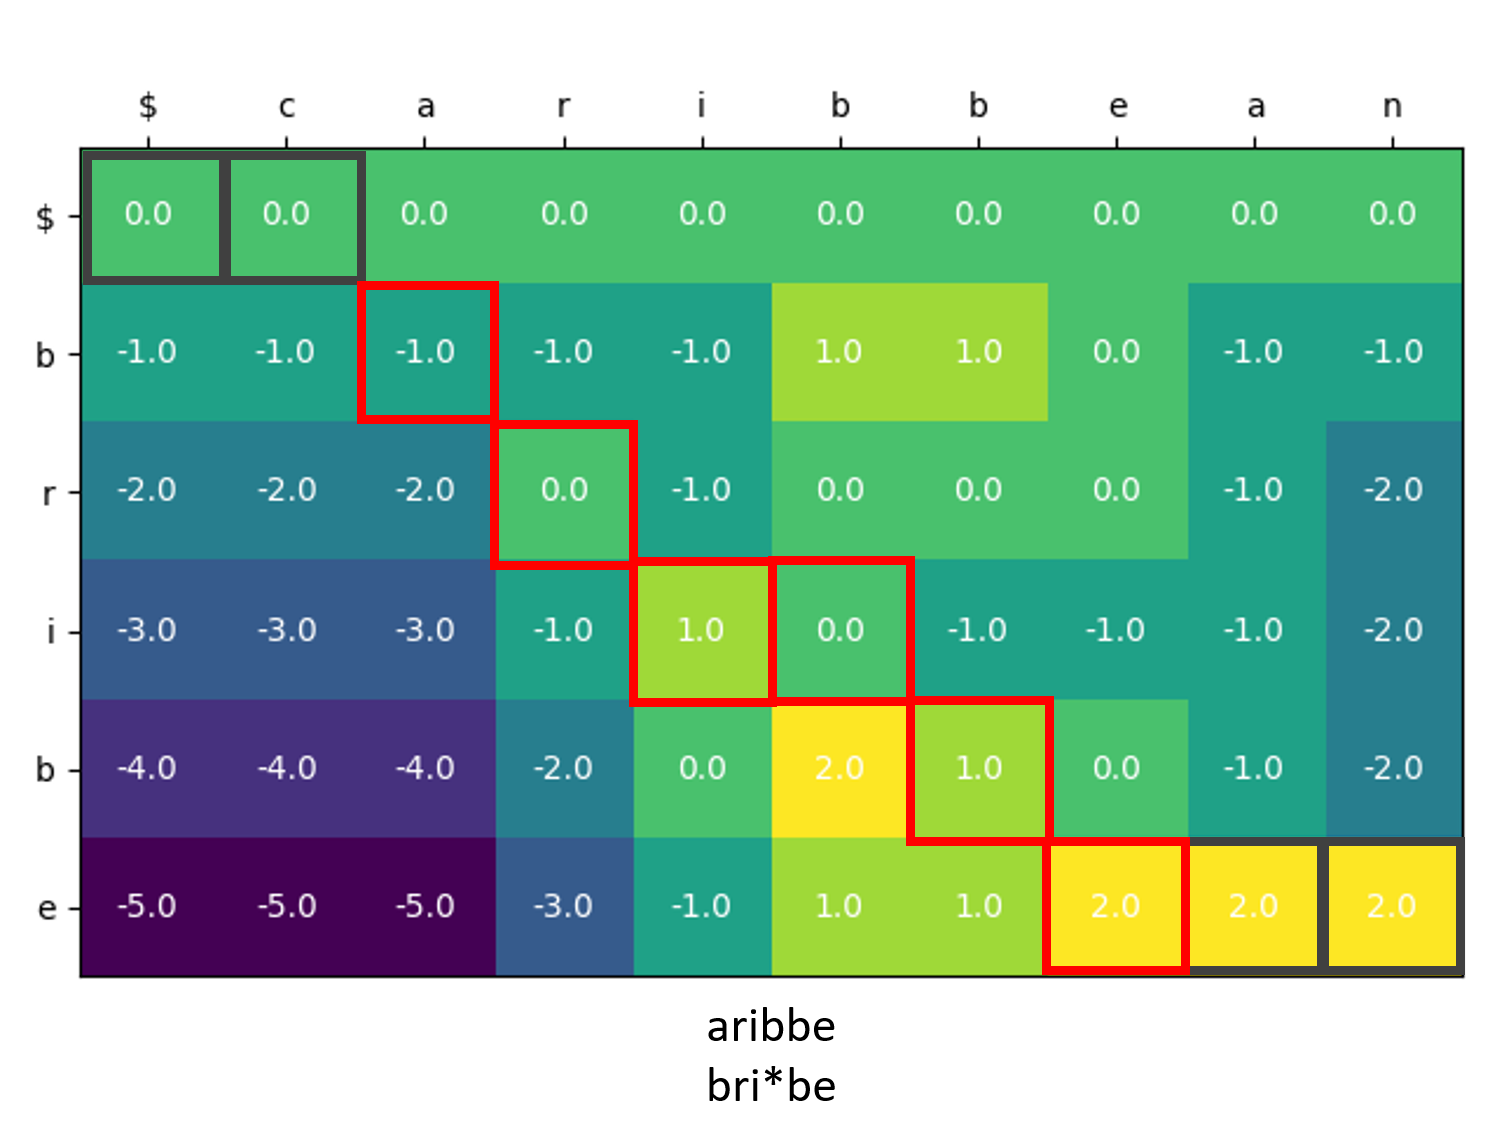
\includegraphics[width=\myPictWidth]{test_needleman_wunsch/caribbean_bribe}
    \caption{Матрица динамического программирования модифицированного алгоритма Нидлмана-Вунша для референса "caribbean"\hspace{0pt} и запроса "bribe". Жирными линиями обведены клетки, соотвтествующие найденному выравниванию }
    \label{fig:caribbean_bribe}
\end{figure}

На рис. \ref{fig:needleman_real} изображены тепловые карты, построенные для образца из реального набора данных. % TODO compare

\begin{figure}[H]
    \centering
    \begin{subfigure}{.5\textwidth}
        \centering
        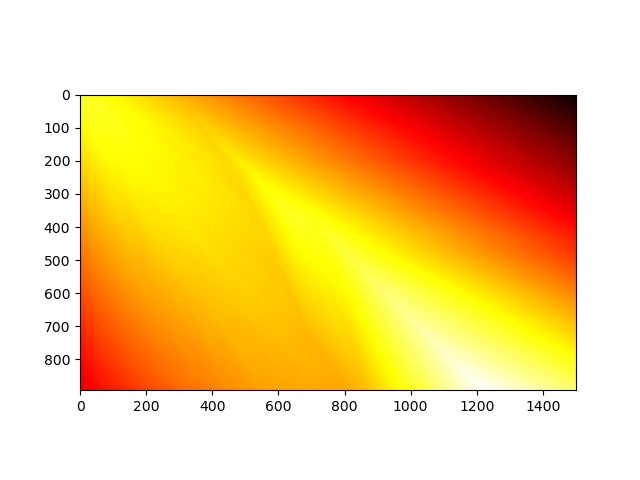
\includegraphics[width=\myPictWidth]{test_needleman_wunsch/big_penalizeTrue}
        \caption{обычный алгоритм}
        \label{fig:needleman_real:usual}
    \end{subfigure}%
    \begin{subfigure}{.5\textwidth}
        \centering
        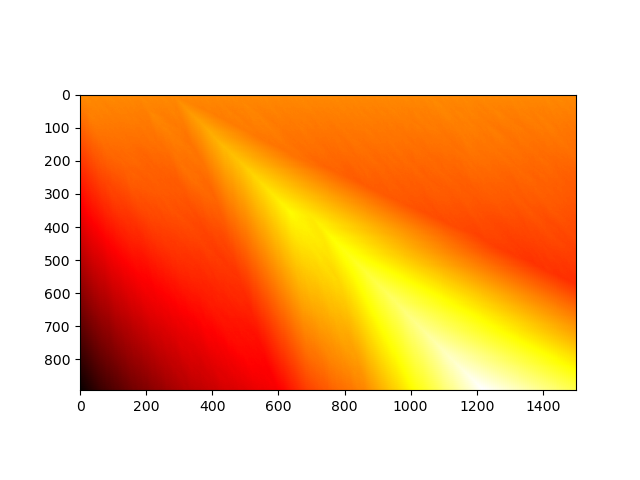
\includegraphics[width=\myPictWidth]{test_needleman_wunsch/big_penalizeFalse}
        \caption{модифицированный алгоритм}
        \label{fig:needleman_real:modified}
    \end{subfigure}
    \caption{Тепловые карты матриц динамического программирования при выравнивании результата распознавания страницы из романа "Scarlet Letter"\hspace{0pt} на участок, найденный с помощью хэширования на референсе.
    Более светлые точки сооветствуют элементам матрицы с большим весом.}
    \label{fig:needleman_real}
\end{figure}

% TODO write about big O complexity

\subsection{Исправление ошибок после выравнивания}

Когда найдено наилучшее соответствие, в запросе исправляются несовпадения и убираются вставки.
При этом учитывается, что в запросе может присутствовать номер страницы и знаки переноса строк, которых нет в референсе (в выравнивании это можно опознать по характерному паттерну: в запросе -- число или знак дефиса с последующим пробелом, в референсной строке -- участок из пропусков).

\subsection{Полуконтролируемое обучение}

Когда метки исправлены, можно провести следующий цикл обучения нейросети, используя аннотированные данные как часть тренировочного набора (в этом и заключается полуконтролируемое обучение).
Как правило, при этом берётся лишь часть данных с псевдометками, отобранная по некоторому критерию качества; в данной работе таким критерием служит доля слов, которые встречаются в исходном тексте.

\end{document}